\section{Quantitative Analysis}
\label{sec:analysis}
%%
%%
In this section, we analyze how we have achieved the main goal of our framework -- reducing storage cost and query workload using transformed distribution data. We have also studied performance of various stages of our framework, and compared our technique with alternate approaches.

\paragraph*{Datasets:} Table~\ref{tbl:datasets} lists the sizes of the datasets used in our experiments. It also presents the size of the integral distribution volume to highlight the huge storage cost associated with it. Loading the entire IDV to memory is not permissible in most cases.
%%
%%%%%%%%%%%%%%%%%%%%%%%%%%%%%%%%%%%%%%%%%
%% Table begins
%%%%%%%%%%%%%%%%%%%%%%%%%%%%%%%%%%%%%%%%%
\begin{table}[!htb]
	\centering	
	\renewcommand{\tabcolsep}{0.09cm}
	\begin{tabular}{|c|c|c|c|}
		\hline
		{\small Dataset} & {\small Size} & {\small Number} & {\small Integral Distribution}\\		
		{\small } & {\small } & {\small of bins} & {\small Volume Size (GB)}\\		
		\hline			
		{\small Plume} & {\small 126x126x512} & {\small 64} & {\small 3.29}\\
		{\small Isabel} & {\small 250x250x50} & {\small 64} & {\small 1.49}\\
		{\small Combustion} & {\small 240x360x60} & {\small 64} & {\small 2.47}\\
		\hline		
	\end{tabular}
	\vspace{-0.3cm}	
	\caption{\label{tbl:datasets} Size of datasets used and the storage cost of corresponding IDVs.}
\end{table}
%%%%%%%%%%%%%%%%%%%%%%%%%%%%%%%%%%%%%%%%%%%%%%%%%%%
%% Table ends
%%%%%%%%%%%%%%%%%%%%%%%%%%%%%%%%%%%%%%%%%%%%%%%%%%%	

For all experiments on all datasets, we have partitioned the data into 1024 blocks and performed both the pre-processing and the query in parallel. Even though our primary focus is not on designing a sophisticated parallel algorithm, we have worked with partitioned data to emphasize the need for our method on large distributed data.

\paragraph*{Alternate Methods:} In terms of storing integral distributions, we have compared against the most straightforward alternative: directly compressing IDV using any off-the-shelf compression scheme. The second alternative is to run the proposed indexing algorithm directly on the IDV, bypassing the decomposition into power-of-two length sub-ranges, and to compress the indexing output. This alternative is presented to justify the importance of the decomposition step in our framework. Finally, we present results from our method which performs decomposition into sub-ranges, then indexing of sub-ranges and finally, compression. 

The third stage -- compression of indexing results -- works with any compression scheme. We have shown results using standard implementations of LZ (Lempel-Ziv)~\cite{lz77} and bzip2 algorithms. Our work does not recommend any particular compression algorithm. Our objective is to transform IDV, which is originally not easy to compress, to an easily compressible form.

In terms of query performance, we have compared against \emph{raw data access} method. Raw data access is a simple load-and-filter approach where, given a range query, each data block that falls within the query is loaded from disk and scanned to compute the partial or full distribution. All these partial distributions are then combined to obtain the final query result. 
%%
%%
\subsection{Space Saving}
\label{sec:analysis_encoding_space}
%%
%%
The primary benefit of our method is that it enables use of integral distributions by reducing its storage cost. When the data is partitioned into $p$ blocks, the \emph{space saving} due to encoding is measured by $\big ( 1 - \frac{\sum_{i=1}^{p} \text{Size of codebook}}{\text{Size of IDV}} \big )$, represented as a percentage. Size of the codebook (for each data block) is the sum of the following: $<$index, transformation$>$ pairs for each sub-range histogram (one integer plus one boolean per histogram), and the compressed residual frequencies after indexing. The utilized templates also need to be stored once for all blocks. To give an idea, the number of templates to be stored for Plume, Isabel and Combustion data are only 403, 249 and 269.

Figure~\ref{fig:spacesaving} presents the space saving obtained by our method and compares it against two other techniques. Space saving for all three methods are measured with respect to the storage cost of the actual IDV. For each group, the leftmost bar indicates the space saving achieved when the IDV is directly compressed using a lossless compression technique such as LZ and bzip2. The middle bar in each group is the result of skipping the sub-range transformation and directly running our indexing algorithm. However, the results indicate that the original distributions from IDV do not lend themselves very well to an indexing algorithm. This justifies the necessity of the transformation into sub-ranges. Finally, we show that our method, combining transformation, indexing and compression, leads to very high space saving (the rightmost bars in each group). 
%%
%%
%%%%%%%%%%%%%%%%%%%
%% Diagram begins
%%%%%%%%%%%%%%%%%%%
\begin{figure}[tb]
\centering
	\subfloat[Compression method used on indexing result: LZ]{\label{fig:spacesaving_lz}
	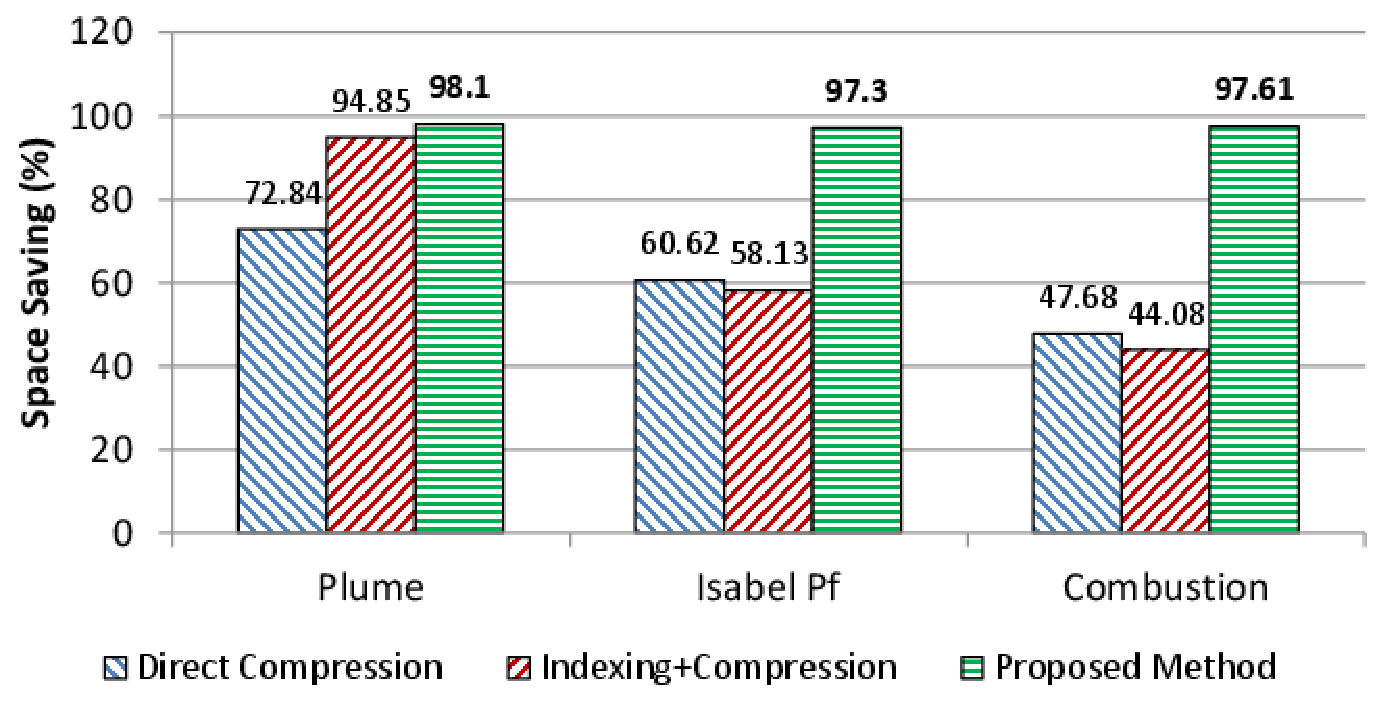
\includegraphics[width = 0.78\linewidth, keepaspectratio = true]{images/eps/spacesaving_lz.eps}}\\
	~
	\subfloat[Compression method used  on indexing result: bzip2]{\label{fig:spacesaving_bz2}
	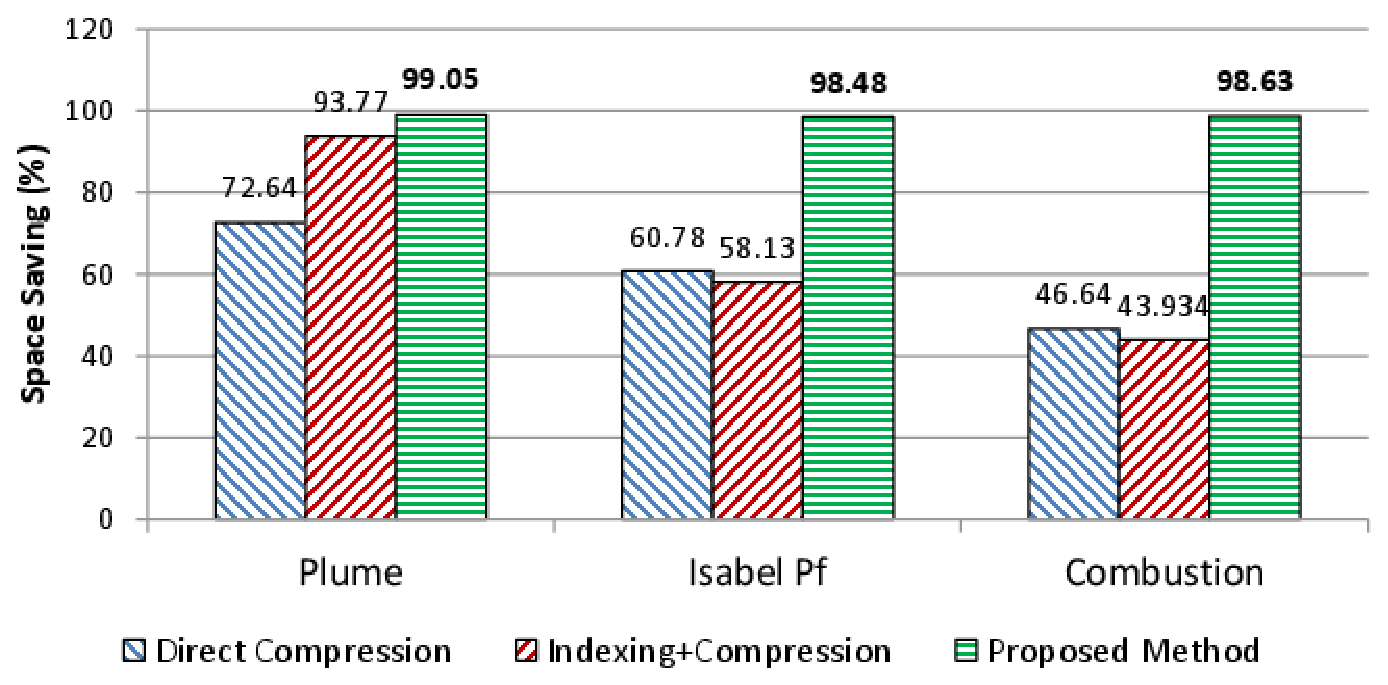
\includegraphics[width = 0.78\linewidth, keepaspectratio = true]{images/eps/spacesaving_bz2.eps}}
	\caption{Space saving achieved by our method (right bars in each group) and two other methods: direct compression of IDV (left bars) and compression after direct indexing of IDV (middle bars).}	
	\label{fig:spacesaving}
\end{figure}
%%%%%%%%%%%%%%%%%%%
%% Diagram ends
%%%%%%%%%%%%%%%%
%%
%%%%%%%%%%%%%%%%%%%%%%%%%%%%%%%%%%%%%%%%%%
%%% Table begins
%%%%%%%%%%%%%%%%%%%%%%%%%%%%%%%%%%%%%%%%%%
%\begin{table}[tb]
%	\centering	
%	\renewcommand{\tabcolsep}{0.09cm}
%	\begin{tabular}{|c|c|c|c|c|}
%		\hline
%		{\small Dataset} & {\small Compression} & \multicolumn{3}{|c|}{\small Space Saving}\\		
%		{\small } & {\small Technique} & \multicolumn{3}{|c|}{\small (\%)}\\		
%		\hline
%		{\small } & {\small } & {\small Direct} & {\small Indexing+} & {\small {\bf Proposed}}\\
%		{\small } & {\small } & {\small Compression}& {\small Compression} & {\small {\bf Method}}\\
%		\hline
%		%{\small } & {\small RLE} & {\small 5.84} & {\small 5.84} & {\small 69.14} & {\small {\bf 91.45}}\\	%5.84301
%		{\small Plume} & {\small LZ} & {\small 72.84} & {\small 94.85} & {\small {\bf 99.14}}\\	%94.85
%		{\small } & {\small BZ2} & {\small 72.64} & {\small 93.77} & {\small {\bf 99.5}}\\		%93.77
%		\hline
%		%{\small } & {\small RLE} & {\small 5.84} & {\small 5.84} & {\small 69.14} & {\small {\bf 91.45}}\\	%5.84301
%		{\small Isabel} & {\small LZ} & {\small 60.62} & {\small 58.13} & {\small {\bf 97.30}}\\	%94.85
%		{\small } & {\small BZ2} & {\small 60.78} & {\small 58.13} & {\small {\bf 98.48}}\\		%93.77
%		\hline
%		%{\small } & {\small RLE} & {\small 5.84} & {\small 5.84} & {\small 69.14} & {\small {\bf 91.45}}\\	%5.84301
%		{\small Combustion} & {\small LZ} & {\small 47.68} & {\small 44.08} & {\small {\bf 97.61}}\\	%94.85
%		{\small } & {\small BZ2} & {\small 46.64} & {\small 43.934} & {\small {\bf 99.5}}\\		%93.77
%		\hline		
%	\end{tabular}
%	\caption{\label{tbl:storagecomp} Storage Reduction by Proposed Technique. Pre-processing is done on 8 processors in parallel. {\bf Isabel and combustion numbers are running}}
%\end{table}
%%%%%%%%%%%%%%%%%%%%%%%%%%%%%%%%%%%%%%%%%%%%%%%%%%%%
%%% Table ends
%%%%%%%%%%%%%%%%%%%%%%%%%%%%%%%%%%%%%%%%%%%%%%%%%%%%	
%%
%%
%%
\subsection{Faster Query Response}
\label{subsec:analysis_encoding_space}
%%
%%
According to our hypothesis, the performance of query in our method should not depend on query size, as we use integral histogram. We have tested this hypothesis by varying the query size from $16^3$ to $48^3$. For each query size, we have used a set of 2000 queries coming from different locations of the data. As shown in Figure~\ref{fig:blockqueryresponse_1}, our method is much faster than the raw data access method for each dataset and across all query sizes. The total time taken by our method always remains less than 0.1 second, while the time taken by raw data access method varies linearly with query size. More importantly, Figure~\ref{fig:blockqueryresponse_2} shows that the speed-up obtained by our method compared to accessing raw data keeps increasing with the query size. This indicates that our method handles larger queries more efficiently, and hence, suits larger datasets.

The above experiment corresponds to the pointwise and blockwise query types. We have also tested the performance of queries whose sizes vary randomly. Each query in the set is a 3D sub-domain centered at the center of the full spatial domain. This allows the query size to vary to the maximum possible extent along each dimension. Figure~\ref{fig:randomqueryresponse} shows that our method provides faster query response (compared to raw data access) for random query as well. The achieved speed-up in total response time for 2000 queries on Plume, Isabel pressure and Combustion dataset are 95.8x, 98.95x and 267x respectively. 

For all our experiments, each dataset is partitioned into 1024 blocks, and the query is computed on 8 processors in parallel. The performance numbers are based on an Intel(R) Core(TM) i7-2600 3.4GHz quad-core processor with 16GB memory.

%Depending on the disk space available, the pre-processed results can be stored as it is, or compressed using some technique. If the data needs to be decompressed during query phase, some computation overhead is added. Hence, for each method, the overhead associated with different compression techniques has been compared.
%%
%%
%%%%%%%%%%%%%%%%%%%
%% Diagram begins
%%%%%%%%%%%%%%%%%%%
\begin{figure}[tb]
\centering	
	\subfloat[Query response time of our method across different query sizes]{\label{fig:blockqueryresponse_1}
	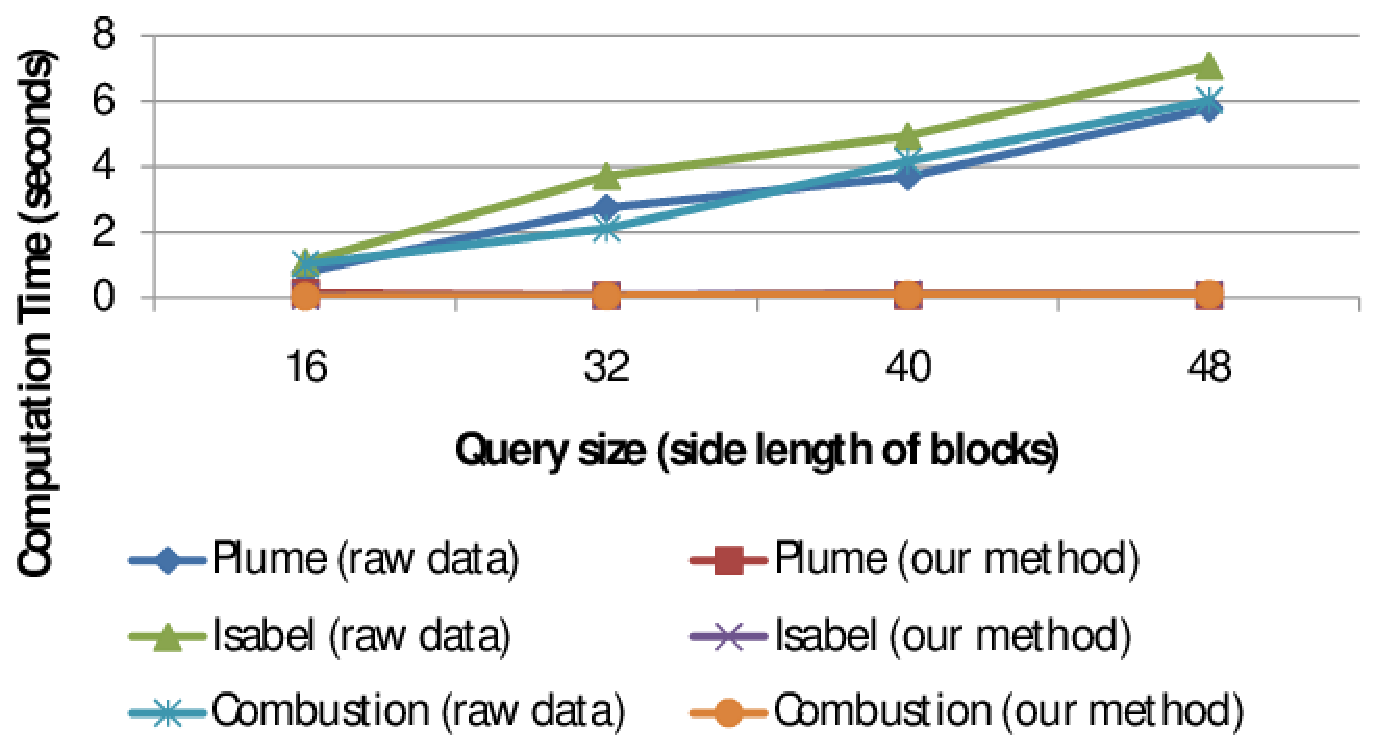
\includegraphics[width = 0.78\linewidth, keepaspectratio = true]{images/eps/block_query_abs.eps}}\\
	\subfloat[Speed-up achieved by our method across different query sizes]{\label{fig:blockqueryresponse_2}
	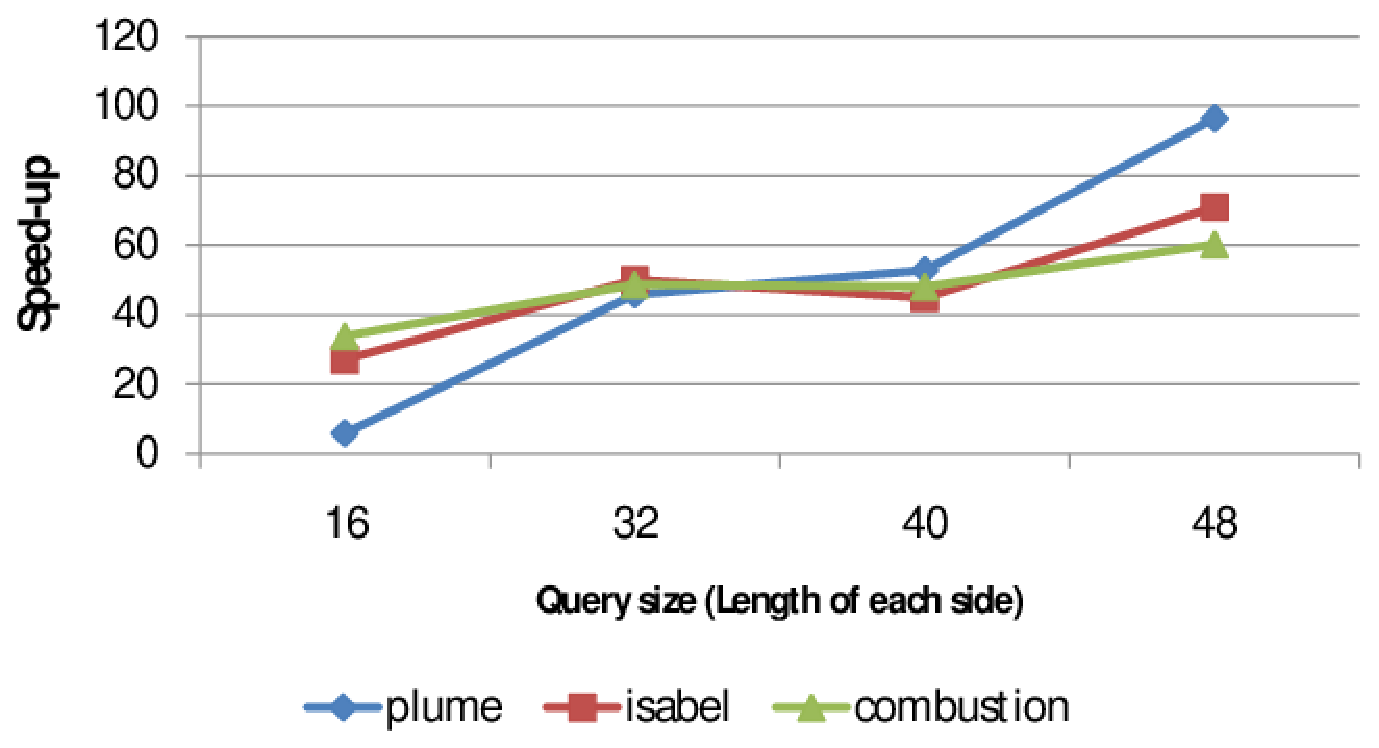
\includegraphics[width = 0.78\linewidth, keepaspectratio = true]{images/eps/block_query_rel.eps}}\\
	\subfloat[Query response time of our method for queries of mixed sizes. Average side length of each query is 101.3 for Plume, 72.66 for Isabel, and 86.84 for Combustion.]{\label{fig:randomqueryresponse}
	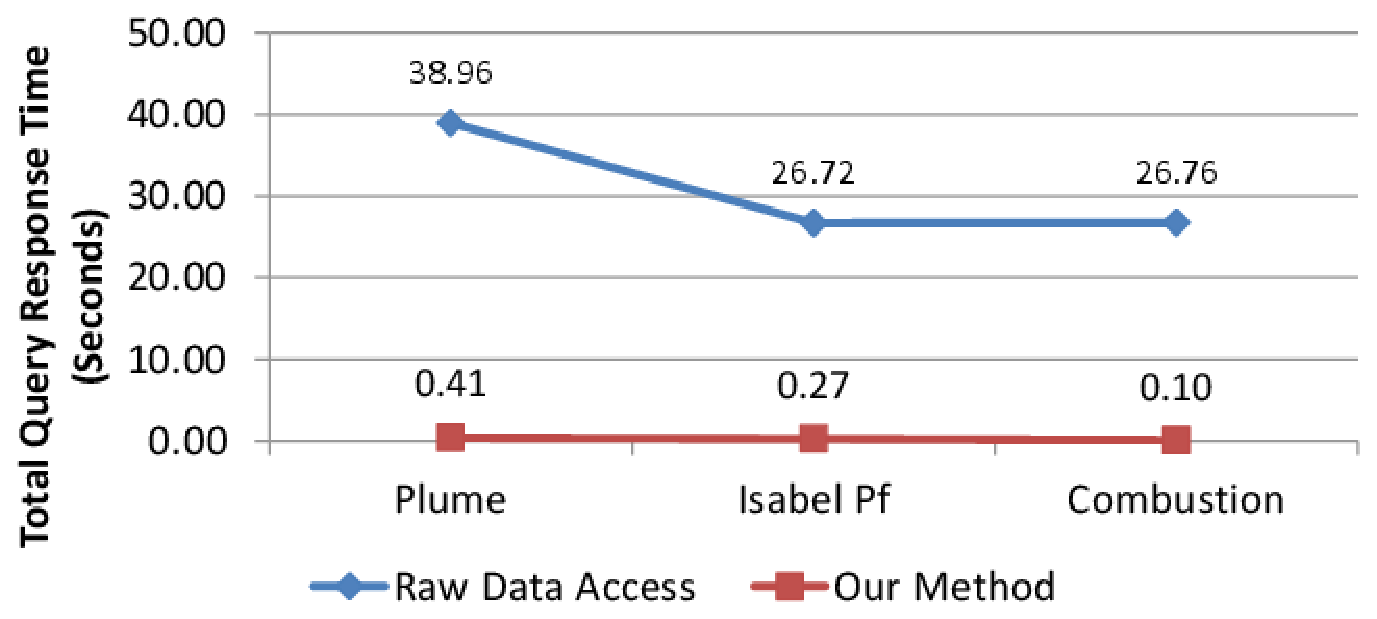
\includegraphics[width = 0.78\linewidth, keepaspectratio = true]{images/eps/random_query.eps}}
	\caption{Performance analysis of query response for different query sizes and different datasets.}	
	\label{fig:queryresponse}
	\vspace{-0.2in}
\end{figure}
%%%%%%%%%%%%%%%%%%%
%% Diagram ends
%%%%%%%%%%%%%%%%
%%
%%
%%%%%%%%%%%%%%%%%%%%%%%%%%%%%%%%%%%%%%%%%%
%%% Table begins
%%%%%%%%%%%%%%%%%%%%%%%%%%%%%%%%%%%%%%%%%%
%\begin{table}[tb]
%	\centering	
%	\renewcommand{\tabcolsep}{0.09cm}
%	\begin{tabular}{|c|c|c|c|c|c|c|}
%		\hline
%		{\small Dataset} & {\small De-comp} & \multicolumn{5}{|c|}{\small Total Query Response Time}\\		
%		{\small } & {\small Technique} & \multicolumn{5}{|c|}{\small (seconds)}\\		
%		\hline
%		{\small } & {\small } & {\small Raw Data} & {\small Direct} & {\small Indexing+} & {\small Compression} & {\small {\bf Proposed}}\\
%		{\small } & {\small } & {\small Access}& {\small comp.} & {\small comp.} & {\small of blocks} & {\small {\bf Method}}\\
%		\hline
%		{\small } & {\small None} & {\small 61.35} & {\small 55.97} & {\small 2.81} & {\small 10.15} & {\small {\bf 12.23}}\\	%5.84301
%		{\small Plume} & {\small LZ} & {\small 0} & {\small 0} & {\small 0} & {\small 0} & {\small {\bf 0}}\\	%94.85
%		{\small } & {\small BZ2} & {\small 0} & {\small 0} &  {\small 0} & {\small 0} & {\small {\bf 0}}\\		%93.77
%		\hline
%		%{\small } & {\small RLE} & {\small 5.84} & {\small 5.84} & {\small 69.14} & {\small {\bf 91.45}}\\	%5.84301
%		{\small Isabel} & {\small LZ} & {\small 0} & {\small 0} & {\small 0} & {\small 0} & {\small {\bf 0}}\\	%94.85
%		{\small } & {\small BZ2} & {\small 0} & {\small 0} & {\small 0} & {\small 0} & {\small {\bf 0}}\\		%93.77
%		\hline
%		%{\small } & {\small RLE} & {\small 5.84} & {\small 5.84} & {\small 69.14} & {\small {\bf 91.45}}\\	%5.84301
%		{\small Combustion} & {\small LZ} & {\small 0} & {\small 0} & {\small 0} & {\small 0} & {\small {\bf 0}}\\	%94.85
%		{\small } & {\small BZ2} & {\small 0} & {\small 0} & {\small 0} & {\small 0} & {\small {\bf 0}}\\		%93.77
%		\hline				
%	\end{tabular}
%	\vspace{-0.3cm}	
%	\caption{\label{tbl:query} Improved Query Response Time by proposed technique. {\bf Isabel and combustion numbers are running}}
%\end{table}
%%%%%%%%%%%%%%%%%%%%%%%%%%%%%%%%%%%%%%%%%%
%%% Table ends
%%%%%%%%%%%%%%%%%%%%%%%%%%%%%%%%%%%%%%%%%%
%
%%
\subsection{Performance Study}
\label{sec:analysis_time}
%%
%%
We have parallelized both the pre-processing and the query stages by partitioning the data into blocks and distributing the blocks across many processors. The pre-processing  (decomposition+indexing+compression) stage is easily adaptable to a parallel framework. In a parallel setting, each processor simultaneously computes its own list of templates based on the blocks assigned to it. A global list of templates is then created by accumulating the local lists. The global list is then distributed back to every processor. A global list is used for indexing because even if two blocks are spatially far apart, they may contain similar distributions. After template creation, each data block is decomposed into sub-ranges and then indexed in its own local co-ordinates space. To compensate for this local transformation, the integral distributions (in global coordinates space) for the corner point, three faces and three edges of the preceding blocks are also stored. Table~\ref{tbl:encodingperf} presents the running times of these stages and the time spent to compress the indexing results for different datasets. 
%%
%%%%%%%%%%%%%%%%%%%%%%%%%%%%%%%%%%%%%%%%%%
%%% Table begins
%%%%%%%%%%%%%%%%%%%%%%%%%%%%%%%%%%%%%%%%%%
\begin{table}[tb]
	\centering	
	\renewcommand{\tabcolsep}{0.09cm}
	\begin{tabular}{|c|c|c|c|c|}
		\hline
		{\small Dataset} & {\small Template} & {\small Sub-range} & {\small Compression} & {\small Compression}\\		
		{\small } & {\small Creation} & {\small Decomposition} & {\small (LZ)} & {\small {BZ2}}\\		
		\hline
		{\small Plume} & {\small 0.26} & {\small 0.09} & {\small 77.49} & {\small 256.02}\\
		{\small Isabel} & {\small 0.07} & {\small 0.04} & {\small 188.59} & {\small 194.77}\\
		{\small Combustion} & {\small 0.09} & {\small 0.07} & {\small 173.899} & {\small 204.262}\\
		\hline				
	\end{tabular}
	\caption{\label{tbl:encodingperf} Performance analysis of different stages of pre-processing (run on 8 processors in parallel). All times are in seconds.}
\end{table}
%%%%%%%%%%%%%%%%%%%%%%%%%%%%%%%%%%%%%%%%%%
%%% Table ends
%%%%%%%%%%%%%%%%%%%%%%%%%%%%%%%%%%%%%%%%%%

The main indexing algorithm is computationally expensive since it compares each sub-range against each template. This is why we have tested the scalability of this stage on Surveyor, an IBM BG/P supercomputer at Argonne National Laboratory. Surveyor contains 1024 quad-core nodes, 2TB memory and utilizes the General Parallel File System (GPFS). Figure~\ref{fig:perf_encoding} shows that the indexing performance scales well with number of processors for all three datasets (each partitioned into 1024 blocks).
%%
%%%%%%%%%%%%%%%%%%%%%%%%%%%%%%%%%%%%%%%%%
%% Figure begins
%%%%%%%%%%%%%%%%%%%%%%%%%%%%%%%%%%%%%%%%%
\begin{figure}[!htb]
\centering
	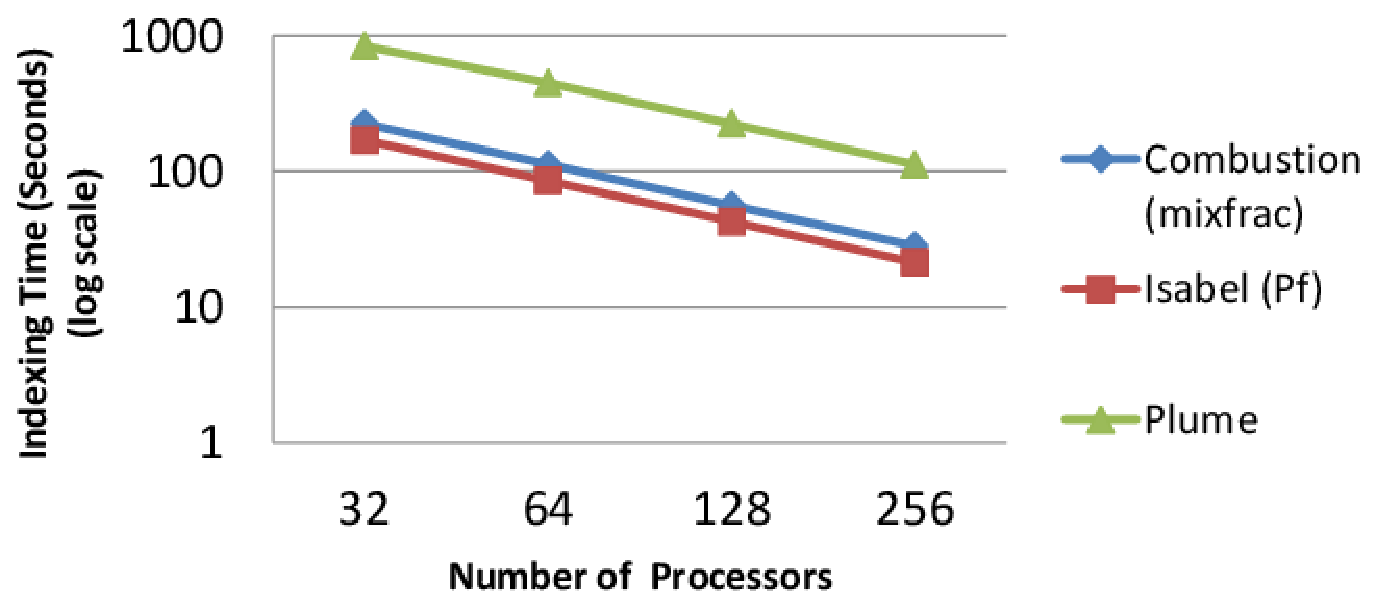
\includegraphics[width = 0.8\linewidth, keepaspectratio = true]{images/eps/perf_encoding.eps}
	\caption{Performance analysis of indexing of power-of-two sub-range distributions from three datasets (each partitioned into 1024 blocks).}	
	\label{fig:perf_encoding}
	\vspace{-0.15in}
\end{figure}
%%%%%%%%%%%%%%%%%%%%%%%%%%%%%%%%%%%%%%%%%%%%%%%%%%%
%% Figure begins
%%%%%%%%%%%%%%%%%%%%%%%%%%%%%%%%%%%%%%%%%%%%%%%%%%%	
%
%%
